\documentclass[tikz]{standalone}
\begin{document}
    \special{background White}
    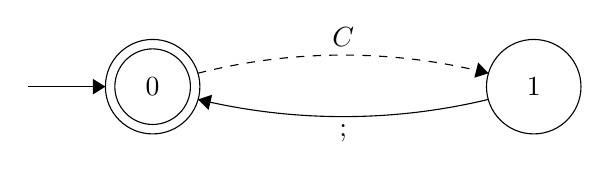
\begin{tikzpicture}[scale=0.2]
        \tikzstyle{every node}+=[inner sep=0pt]
        \draw [black] (23.6,-31.7) circle (3);
        \draw (23.6,-31.7) node {$0$};
        \draw [black] (23.6,-31.7) circle (2.4);
        \draw [black] (47.8,-31.7) circle (3);
        \draw (47.8,-31.7) node {$1$};
        \draw [black] (15.7,-31.7) -- (20.6,-31.7);
        \fill [black] (20.6,-31.7) -- (19.8,-31.2) -- (19.8,-32.2);
        \draw [dashed] (26.475,-30.846) arc (104.25327:75.74673:37.468);
        \fill [black] (44.93,-30.85) -- (44.27,-30.16) -- (44.03,-31.13);
        \draw (35.7,-29.19) node [above] {$C$};
        \draw [black] (44.913,-32.511) arc (-76.48764:-103.51236:39.428);
        \fill [black] (26.49,-32.51) -- (27.15,-33.18) -- (27.38,-32.21);
        \draw (35.7,-34.1) node [below] {$;$};
    \end{tikzpicture}
\end{document}
